\documentclass[aspectratio=169,10pt]{beamer}

\usetheme{Madrid}
\usecolortheme{seahorse}

\usepackage[utf8]{inputenc}
\usepackage{amsmath, amssymb, amsfonts}
\usepackage{mathtools}
\usepackage{graphicx}
\usepackage{xcolor}
\usepackage{listings}
\usepackage{xfrac}
\usepackage{array}
\usepackage{booktabs}

% Configure listings for code
\lstset{
    basicstyle=\ttfamily\scriptsize,
    commentstyle=\color{green!50!black}\itshape,
    keywordstyle=\color{blue}\bfseries,
    stringstyle=\color{red},
    breaklines=true,
    frame=single,
    numbers=left,
    numberstyle=\tiny\color{gray},
    showstringspaces=false,
    language=Python
}

% Path to figures
\graphicspath{{figures/}}

% Configure footer
\setbeamertemplate{footline}[frame number]

% Define colors for overlays
\definecolor{darkblue}{RGB}{25,50,100}
\definecolor{darkgreen}{RGB}{34,120,34}
\definecolor{darkred}{RGB}{139,0,0}

\title[Chapter 10a: Set-Valued Mappings]{Chapter 10a: Set-Valued Mappings}
\subtitle{Applications of Fixed Point Theorems for Multifunctions to Integral Inclusions}
\author{Pathak, H.K. \\ \textit{An Introduction to Nonlinear Analysis and Fixed Point Theory}}
\institute{Pathak's Textbook, 2018}
\date{2024}

\begin{document}

\frame{\titlepage}

% ============================================================================
% TABLE OF CONTENTS
% ============================================================================

\begin{frame}
\frametitle{Contents}
\tableofcontents
\end{frame}

% ============================================================================
% SECTION 1: INTRODUCTION TO SET-VALUED MAPPINGS
% ============================================================================

\section{Introduction to Set-Valued Mappings}

\begin{frame}
\frametitle{What is a Set-Valued Mapping?}

\begin{definition}[Set-Valued Mapping]
A \textbf{multivalued mapping} (or \textbf{set-valued map}) is a function
\[
F: X \to \mathcal{P}(Y)
\]
where $\mathcal{P}(Y)$ denotes the \textit{power set} of $Y$ (the collection of all subsets of $Y$).

For each point $x \in X$, we have a \textbf{nonempty subset} $F(x) \subseteq Y$.
\end{definition}

\vspace{0.5cm}

\textbf{Key difference from single-valued mappings:}
\begin{itemize}
    \item Single-valued: $f: X \to Y$ maps each $x$ to a single point $f(x)$
    \item Set-valued: $F: X \to \mathcal{P}(Y)$ maps each $x$ to a \textit{set} $F(x)$
\end{itemize}

\vspace{0.5cm}

\textbf{Applications:}
\begin{itemize}
    \item Differential inclusions and optimal control
    \item Variational inequalities
    \item Game theory and economics
    \item Integral inclusions
\end{itemize}

\end{frame}

\begin{frame}
\frametitle{Visual Representation of Set-Valued Mappings}

\begin{center}
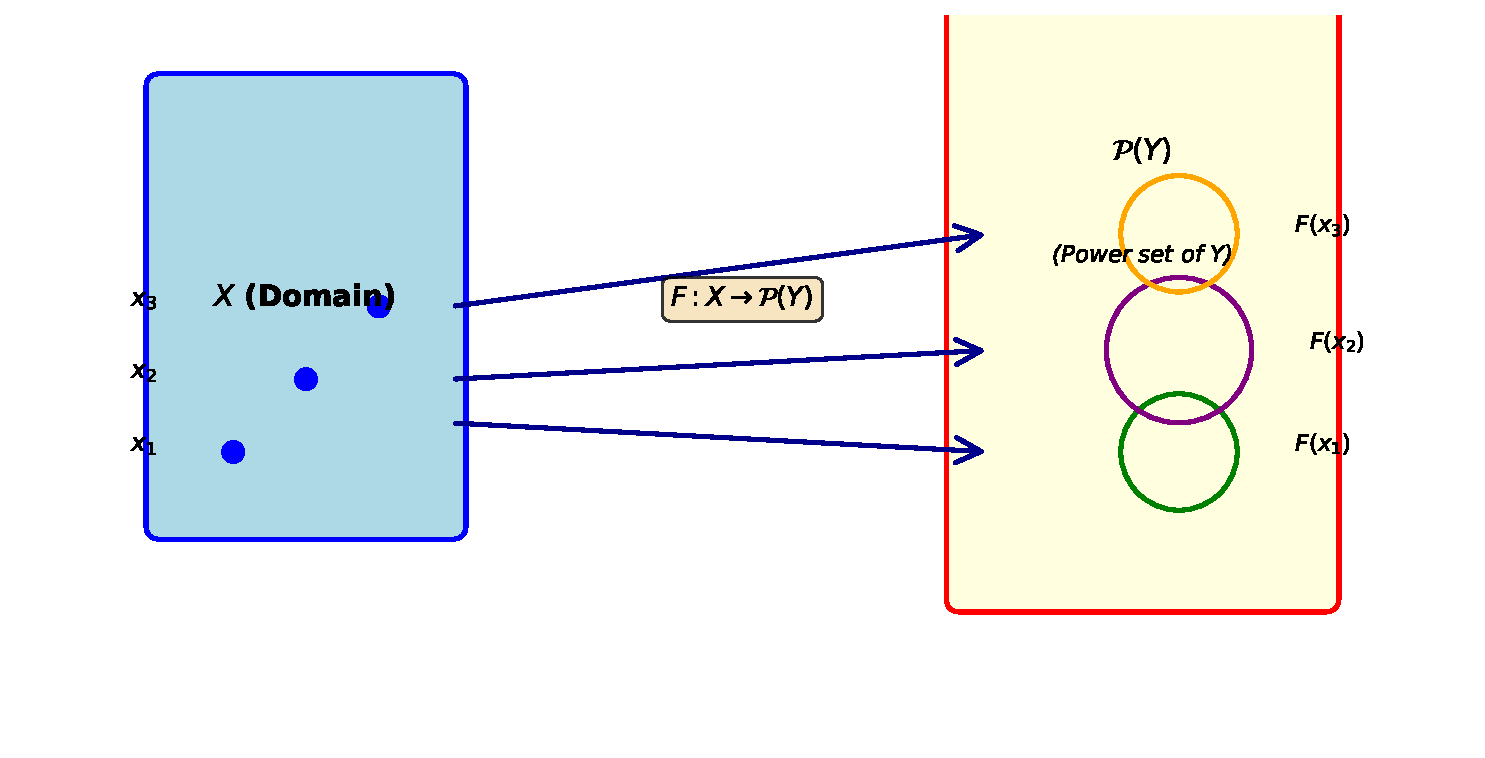
\includegraphics[height=0.75\textheight]{set_valued_mapping}
\end{center}

\end{frame}

\begin{frame}
\frametitle{Types of Set-Valued Mappings}

\begin{definition}[Upper Semicontinuity]
A set-valued map $F: X \to \mathcal{P}(Y)$ is \textbf{upper semicontinuous} (u.s.c.) at $x_0$ if for every open set $V$ with $F(x_0) \subseteq V$, there exists an open neighborhood $U$ of $x_0$ such that $F(x) \subseteq V$ for all $x \in U$.
\end{definition}

\begin{definition}[Lower Semicontinuity]
$F$ is \textbf{lower semicontinuous} (l.s.c.) at $x_0$ if for every open set $V$ with $F(x_0) \cap V \neq \emptyset$, there exists an open neighborhood $U$ of $x_0$ such that $F(x) \cap V \neq \emptyset$ for all $x \in U$.
\end{definition}

\vspace{0.3cm}

\textbf{Other important properties:}
\begin{itemize}
    \item \textbf{Compactness}: $F(x)$ is a compact set for each $x \in X$
    \item \textbf{Convexity}: $F(x)$ is a convex set for each $x \in X$
    \item \textbf{Closedness}: $F(x)$ is closed for each $x \in X$
    \item \textbf{Measurability}: For suitable function spaces
\end{itemize}

\end{frame}

\begin{frame}
\frametitle{Properties of Multivalued Operators}

\begin{center}
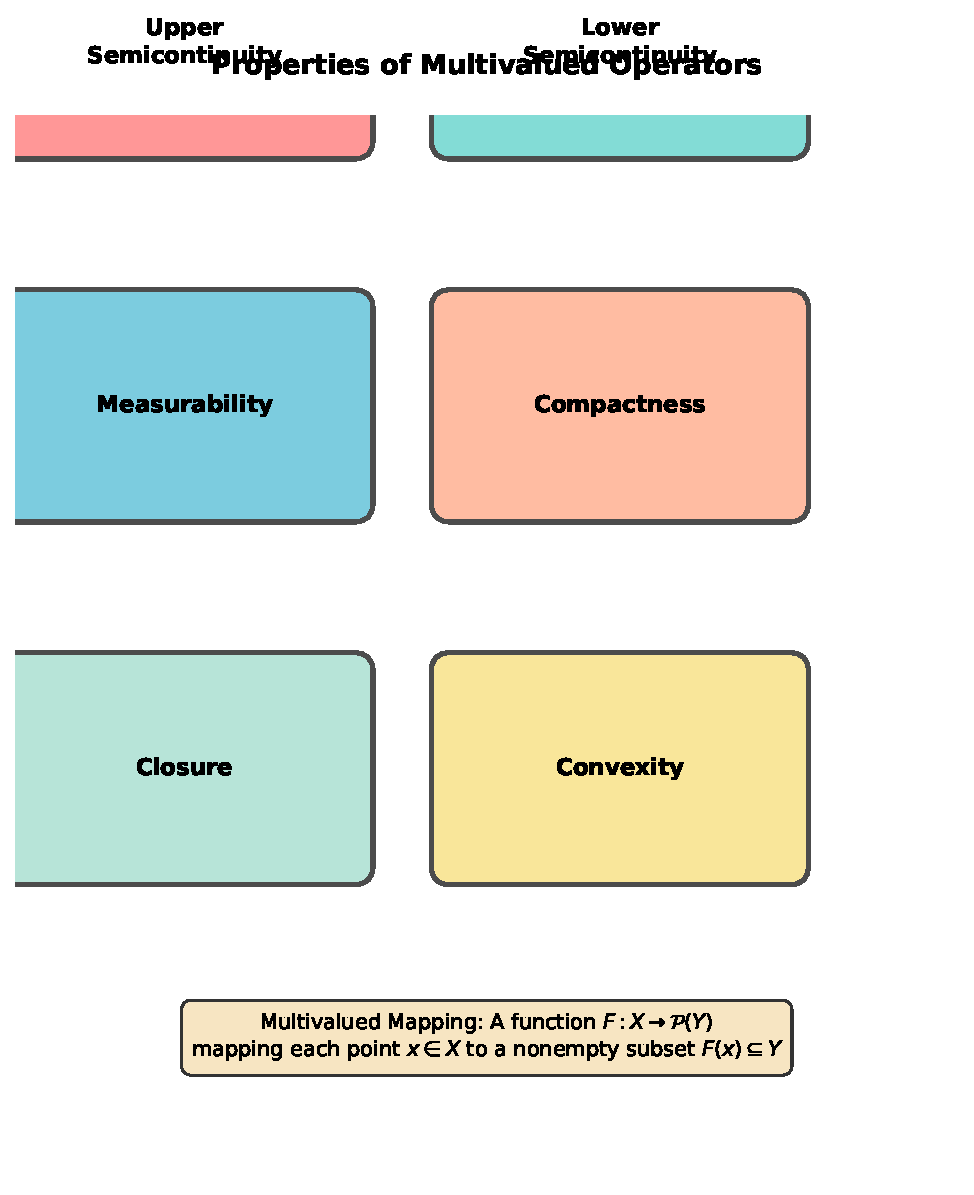
\includegraphics[height=0.75\textheight]{multivalued_properties}
\end{center}

\end{frame}

% ============================================================================
% SECTION 2: NEMYTSKII OPERATORS AND INTEGRAL INCLUSIONS
% ============================================================================

\section{Nemytskii Operators and Integral Inclusions}

\begin{frame}
\frametitle{Nemytskii Operators}

\begin{definition}[Nemytskii Operator]
Given a set-valued mapping $f: [0,T] \times \mathbb{R} \to \mathcal{P}(\mathbb{R})$, the \textbf{Nemytskii operator} is defined as:
\[
N_f(u) = \left\{y \in L^p[0,T] : y(t) \in f(t, u(t))\ \text{a.e.}\ t \in [0,T]\right\}
\]
\end{definition}

\vspace{0.5cm}

\begin{center}
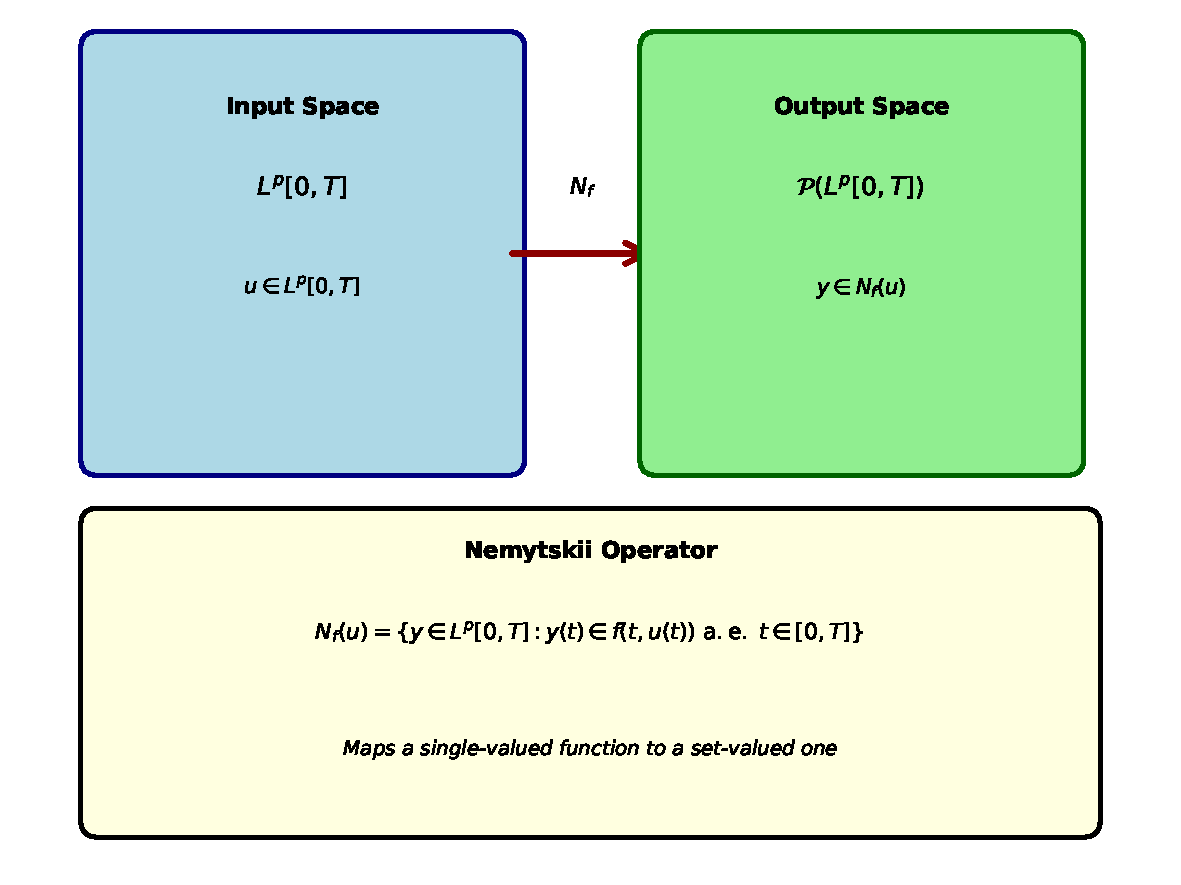
\includegraphics[height=0.5\textheight]{nemytskii_operator}
\end{center}

\textbf{Significance:} Nemytskii operators convert function spaces of single-valued mappings into function spaces of set-valued mappings.

\end{frame}

\begin{frame}
\frametitle{Integral Inclusions: Basic Framework}

\begin{definition}[Fredholm Integral Inclusion]
A \textbf{Fredholm integral inclusion} is of the form:
\[
y(t) \in \int_0^T k(t,s) A(s, y(s)) \, ds \quad \text{a.e. } t \in [0,T]
\]
where:
\begin{itemize}
    \item $k(t,s)$ is a kernel function
    \item $A(t,y)$ is a set-valued map
    \item The integral is interpreted in the sense of set-valued analysis
\end{itemize}
\end{definition}

\vspace{0.5cm}

\textbf{Reduction to Operator Equation:}
\[
y \in A_{\kappa}(y) \quad \text{for some } y \in L^p[0,T]
\]

This is a \textbf{fixed point problem} for the multivalued operator $A_{\kappa}$.

\end{frame}

\begin{frame}
\frametitle{Structure of Integral Inclusions}

\begin{center}
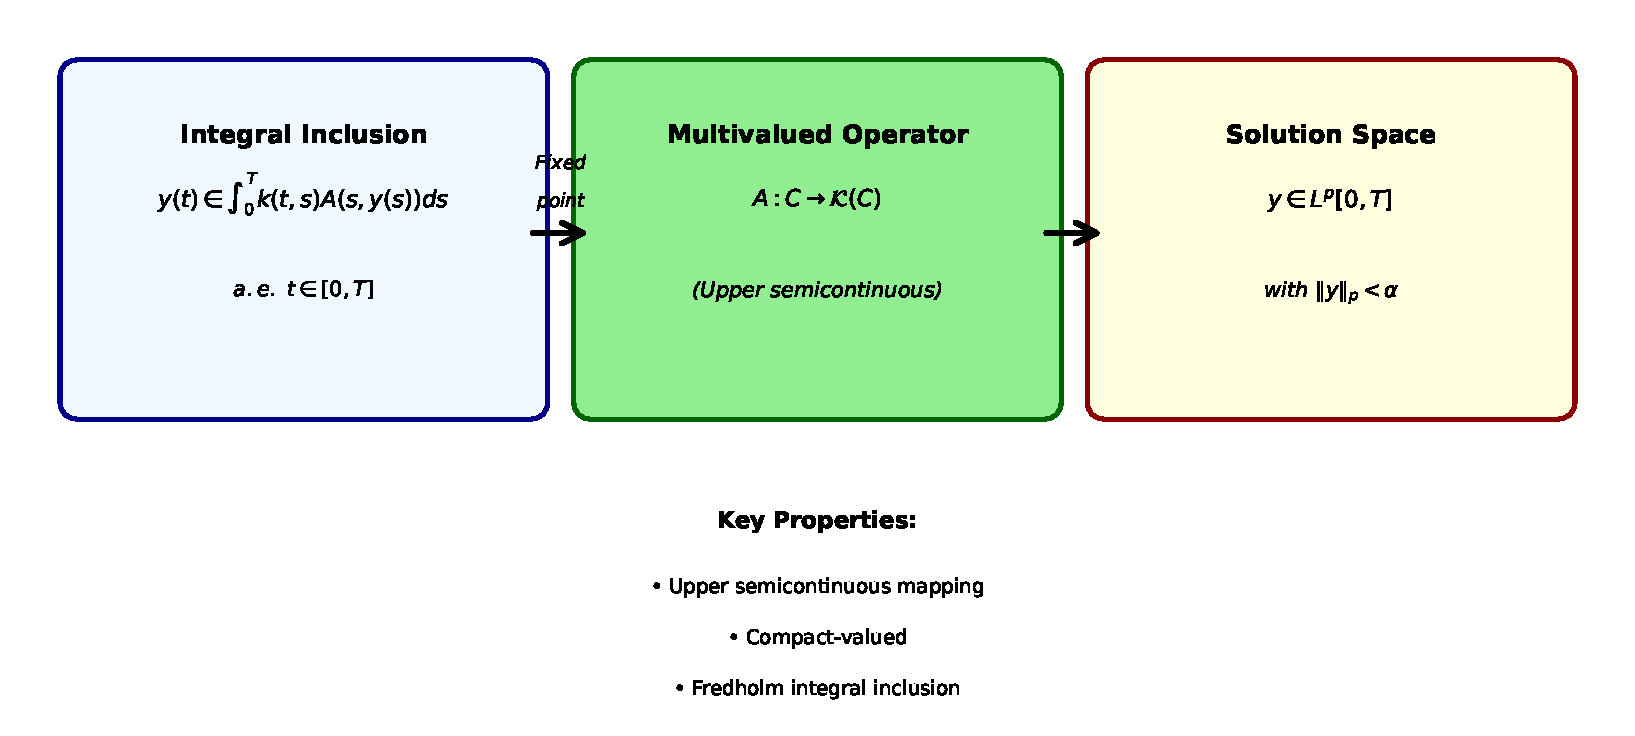
\includegraphics[height=0.75\textheight]{integral_inclusion_structure}
\end{center}

\end{frame}

% ============================================================================
% SECTION 3: CONTINUOUS SOLUTIONS TO NONLINEAR INTEGRAL INCLUSIONS
% ============================================================================

\section{Continuous Solutions for Nonlinear Integral Inclusions}

\begin{frame}
\frametitle{Fredholm Integral Inclusion with General Setup}

Consider the problem:
\[
\begin{cases}
y(t) \in a(t)g(s, u(s)) + \tilde{f}(s, u(s), u'(s)) & \text{a.e. } s \in [0, T] \\
\sup_{s \in [0,T]} |u'(s)| \leq \lambda &
\end{cases}
\]

\vspace{0.5cm}

\begin{theorem}[Theorem 10.1 - Existence of Continuous Solutions]
Let $(X, A, \mu)$ be a finite measure space and $X$ a Banach space. Suppose:
\begin{enumerate}
    \item $y(s) \in a(s)g(s, u(s)) + \tilde{f}(s, u(s), u'(s))$ for measurable $a$, $g$, $\tilde{f}$
    \item $N_f : L_p[0,T] \to 2^{L_p[0,T]}$ is the generalized Nemytskii operator
    \item Define $Ay = \{y \in L^p[0,T] : y(t) \in \int_0^T k(t,s)y(s)\,ds\}$
\end{enumerate}

Then the operator $A: C \to 2^C$ is \textbf{upper semicontinuous and compact}.
\end{theorem}

\end{frame}

\begin{frame}
\frametitle{Key Properties for Existence}

For the integral inclusion to have a solution, we need:

\vspace{0.3cm}

\begin{enumerate}
    \item \textbf{Upper Semicontinuity} of $A$:
    \[
    A: C \to \mathcal{K}(C) \text{ is u.s.c.}
    \]
    where $\mathcal{K}(C)$ is the collection of nonempty compact subsets of $C$.

    \vspace{0.3cm}

    \item \textbf{Compactness}: The operator maps to compact-valued sets.

    \vspace{0.3cm}

    \item \textbf{Growth Bounds}: For $x \in C \cap \partial\Omega_\alpha$:
    \[
    \|y\|_p < \|x\|_p \quad \text{for } y \in Ax
    \]
    \[
    \|y\|_p > \|x\|_p \quad \text{for } x \in C \cap \partial\Omega_\beta
    \]
\end{enumerate}

\vspace{0.5cm}

These ensure by \textbf{Theorem 5.167} (multivalued fixed point theorem) that $A$ has a fixed point.

\end{frame}

\begin{frame}
\frametitle{Example: C[0,T] Solutions}

\begin{definition}[C[0,T] Problem]
Consider the Fredholm integral inclusion:
\[
y(t) \in \int_0^T k(t,s)[a(t,s)g(t, y(s)) + \tilde{f}(t, s, y(s))] \, ds \quad \text{a.e. } t \in [0,T]
\]
with finite derivative at each $s \in [0,T]$.
\end{definition}

\vspace{0.5cm}

\begin{theorem}[Theorem 10.2]
Let $1 \leq p < \infty$ and $q$ be conjugate to $p$. Assume:
\begin{enumerate}
    \item For each $t \in [0,T]$, the map $s \mapsto k(t,s)$ is measurable
    \item $\tilde{f}: [0,T]^2 \times \mathbb{R} \to \mathcal{K}(\mathbb{R})$ is measurable
    \item Growth and Lipschitz conditions are satisfied
\end{enumerate}

Then there exists a nonnegative solution $y \in C[0,T]$ to the integral inclusion.
\end{theorem}

\end{frame}

\begin{frame}[fragile]
\frametitle{Numerical Example: Integral Inclusion Solution}

\begin{lstlisting}
import numpy as np
from scipy.integrate import odeint
import matplotlib.pyplot as plt

# Parameters
T = 1.0
t = np.linspace(0, T, 100)

# Kernel function
def kernel(t, s):
    return np.exp(-(t - s)**2)

# Set-valued mapping (example)
def f(t, y):
    # Returns interval [a(t,y), b(t,y)]
    a = -0.1 * y - 0.5
    b = 0.1 * y + 0.5
    return a, b

# Compute integral inclusion solution
y_solution = np.zeros_like(t)
for i, t_i in enumerate(t):
    integral = 0.0
    for j, s_j in enumerate(t):
        k_val = kernel(t_i, s_j)
        # Take midpoint of f(s_j, y[j])
        f_val = np.mean(f(s_j, y_solution[j]))
        integral += k_val * f_val * (t[1] - t[0])
    y_solution[i] = integral

# Plot solution
plt.figure(figsize=(10, 6))
plt.plot(t, y_solution, 'b-', linewidth=2, label='Solution $y(t)$')
plt.xlabel('Time $t$', fontsize=12)
plt.ylabel('$y(t)$', fontsize=12)
plt.title('Solution to Fredholm Integral Inclusion', fontsize=13)
plt.legend(fontsize=11)
plt.grid(True, alpha=0.3)
plt.tight_layout()
plt.savefig('integral_solution.png', dpi=150)
\end{lstlisting}

\end{frame}

% ============================================================================
% SECTION 4: HAMMERSTEIN TYPE INTEGRAL INCLUSIONS
% ============================================================================

\section{Hammerstein Type Integral Inclusions}

\begin{frame}
\frametitle{Hammerstein Integral Inclusions}

\begin{definition}[Hammerstein Type Problem]
The \textbf{nonconvex Hammerstein integral inclusion} is:
\[
x(t) = \lambda(t) + \int_0^T k(t,s) F(s, V(x)(s)) \, ds
\]
where:
\begin{itemize}
    \item $\lambda: [0,T] \to X$ is a continuous function
    \item $F: I \times X \to \mathcal{P}(X)$ is a set-valued map
    \item $V: C(I,X) \to C(I,X)$ is a single-valued operator
    \item $k(t,s)$ is the kernel function
\end{itemize}
\end{definition}

\vspace{0.5cm}

\textbf{Applications:}
\begin{itemize}
    \item Control systems governed by parabolic PDEs
    \item Differential inclusions in Banach spaces
    \item Existence of mild solutions to evolution equations
\end{itemize}

\end{frame}

\begin{frame}
\frametitle{Semigroup Framework}

\begin{definition}[C₀-Semigroup]
A family $\{G(t) : t \in \mathbb{R}^+\}$ of bounded linear operators from $X$ into $E$ is a \textbf{$C_0$-semigroup} (linear semigroup of class $C_0$) on $X$ if:
\begin{enumerate}
    \item $G(0) = I$ (identity operator)
    \item $G(t+s) = G(t)G(s)$ for all $t, s \geq 0$ (semigroup property)
    \item $G(\cdot)$ is strongly continuous in $t \in \mathbb{R}^+$
    \item $\|G(t)\| \leq M e^{\omega t}$ for some $M > 0$ and $\omega \in \mathbb{R}$
\end{enumerate}
\end{definition}

\vspace{0.5cm}

\textbf{Significance:} Semigroups provide a framework for studying evolution equations and their solutions in infinite-dimensional Banach spaces.

\end{frame}

\begin{frame}
\frametitle{Example: Parabolic PDE as Hammerstein Inclusion}

\begin{example}
Consider the parabolic system:
\[
\begin{cases}
x'(t) = Ax(t) + F(t, x(t)) & t \in [0,T] \\
x(0) = x_0
\end{cases}
\]

where $A$ is the infinitesimal generator of a $C_0$-semigroup $\{G(t)\}_{t \geq 0}$ and $F$ is a set-valued map.

A \textbf{mild solution} is:
\[
x(t) = G(t)x_0 + \int_0^t G(t-s)f(s) \, ds
\]
where $f(s) \in F(s, x(s))$ a.e.
\end{example}

\vspace{0.5cm}

This is a special case of the Hammerstein integral inclusion with $\lambda(t) = G(t)x_0$ and $V(x)(s) = x(s)$.

\end{frame}

\begin{frame}
\frametitle{Existence for Hammerstein Inclusions}

\begin{theorem}[Existence for Hammerstein Inclusions]
Assume:
\begin{enumerate}
    \item $F: I \times X \to \mathcal{P}(X)$ has nonempty closed values
    \item $F$ is measurable and satisfies an L-Lipschitz condition
    \item $V: C(I,X) \to C(I,X)$ has continuity and boundedness properties
    \item $k(t,s)$ satisfies suitable boundedness conditions
\end{enumerate}

Then there exists a solution $x \in C(I, X)$ to the Hammerstein integral inclusion.
\end{theorem}

\vspace{0.5cm}

\textbf{Key Steps:}
\begin{enumerate}
    \item Define the solution operator: $Tx(t) = \lambda(t) + \int_0^t k(t,s)F(s,V(x)(s))\,ds$
    \item Verify $T$ is upper semicontinuous and compact
    \item Apply Theorem 5.167 (multivalued fixed point theorem)
    \item Obtain solution as fixed point of $T$
\end{enumerate}

\end{frame}

% ============================================================================
% SECTION 5: FILIPPOV TYPE EXISTENCE THEOREM
% ============================================================================

\section{Filippov Type Existence Theorem}

\begin{frame}
\frametitle{Filippov Type Integral Inclusions}

\begin{definition}[Filippov Problem]
The \textbf{Filippov type integral inclusion} is:
\[
u(t) \in F(t, V(x(t))) \quad \text{a.e. } (I := [0,T])
\]
where:
\begin{itemize}
    \item $\lambda(\cdot): I \to X$ is a given mapping
    \item $g(\cdot, \cdot): I \times X \to X$ is continuous
    \item $F(\cdot, \cdot): I \times X \to \mathcal{P}(X)$ is set-valued
    \item $f(\cdot, \cdot, \cdot): I \times I \times X \to X$ is continuous
    \item $V: C(I,X) \to C(I,X)$ is continuous
\end{itemize}
\end{definition}

\vspace{0.5cm}

\textbf{Connection to Control Systems:}
Filippov's theorem addresses differential inclusions arising from control problems:
\[
x'(t) \in F(t, x(t)), \quad x(0) = x_0
\]
where $F$ is upper semicontinuous with closed, convex values.

\end{frame}

\begin{frame}
\frametitle{Main Assumptions for Filippov Theorem}

\begin{hypothesis}[Hypothesis 10.2]
Let $F(\cdot, \cdot): I \times X \to \mathcal{P}(X)$ be a set-valued map with nonempty closed values that:

\begin{enumerate}
    \item[(H₁)] $F(\cdot, \cdot)$ is $\mathcal{L}(I) \otimes \mathcal{B}(X)$ measurable

    \item[(H₂)] $\exists L(\cdot) \in L_1(I, \mathbb{R}^+)$ such that $F(t, \cdot)$ is $L(t)$-Lipschitz:
    \[
    H^+(F(t,x), F(t,y)) \leq L(t)\|x - y\| \quad \forall x,y \in X
    \]

    \item[(H₃)] For $\sigma \in L_1(I,E)$ and $T_\sigma(t)$ the solution set:
    \[
    d(\psi_1, T_\lambda(\sigma_2)) \leq H^+(T_\lambda(\sigma_1), T_\lambda(\sigma_2))
    \]

    \item[(H₄)] $a: I \times I \to \mathbb{R}$ is continuous satisfying Hölder's continuity condition
\end{enumerate}

\end{hypothesis}

\end{frame}

\begin{frame}
\frametitle{Filippov Existence Theorem}

\begin{theorem}[Theorem 10.3 - Filippov Type Existence]
Under Hypothesis 10.2, if $\sup_{t \in I}\|u_0(t)\|$ is bounded and the system parameters satisfy growth and Lipschitz conditions, then the Filippov type integral inclusion admits at least one solution pair $(x,u)$ where:
\begin{itemize}
    \item $x(\cdot) \in C(I, X)$ is the state trajectory
    \item $u(\cdot) \in L^1(I, X)$ is the control (selection from $F$)
\end{itemize}
\end{theorem}

\vspace{0.5cm}

\textbf{Proof Strategy:}
\begin{enumerate}
    \item Reformulate as fixed point problem: $x = Tx$ for appropriate operator $T$
    \item Prove $T$ is upper semicontinuous with compact, convex values
    \item Establish a priori bounds on solutions
    \item Apply Leray-Schauder alternative theorem
\end{enumerate}

\end{frame}

\begin{frame}
\frametitle{Fundamental Results and Tools}

\begin{center}
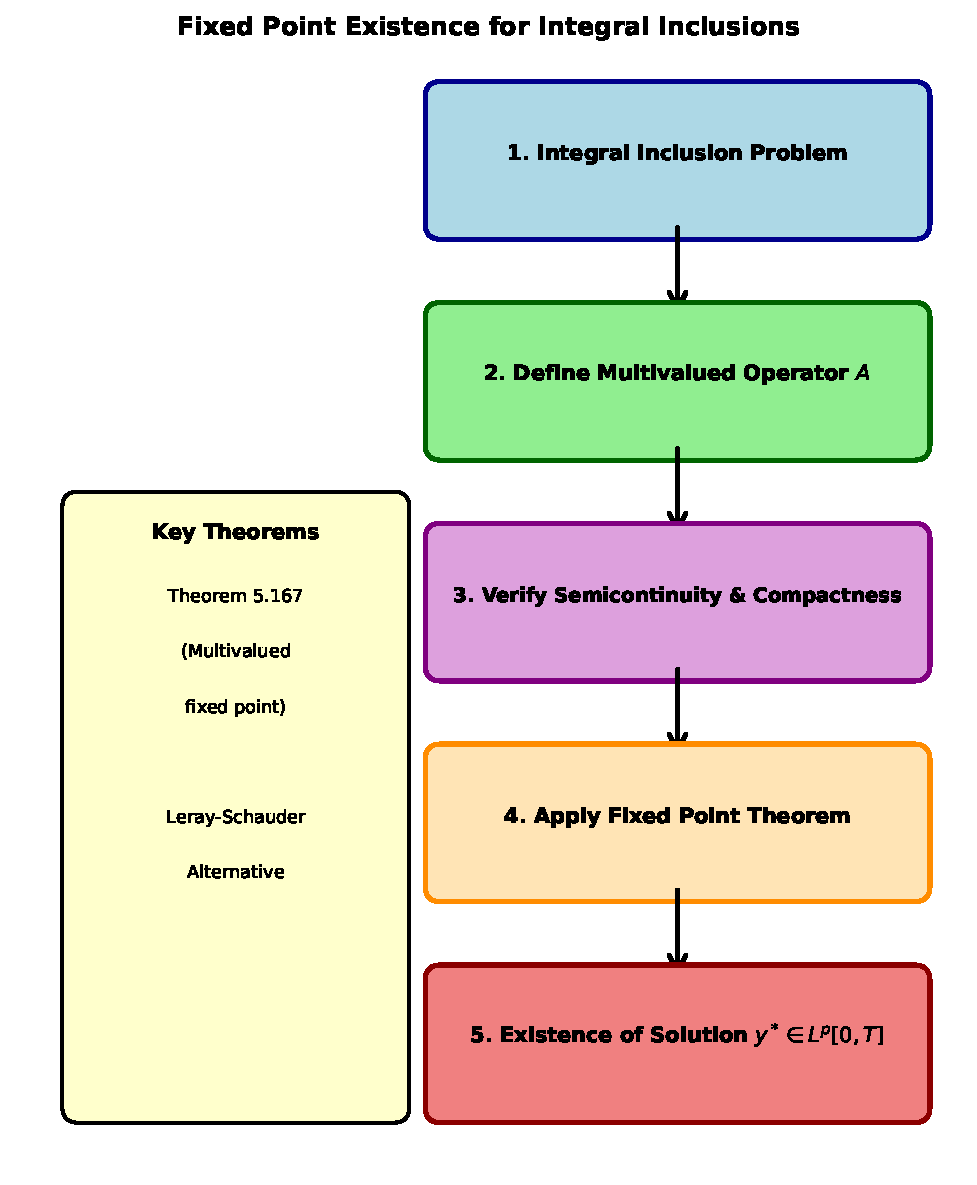
\includegraphics[height=0.75\textheight]{fixed_point_existence_flow}
\end{center}

\end{frame}

% ============================================================================
% SECTION 6: APPLICATIONS AND EXAMPLES
% ============================================================================

\section{Applications and Examples}

\begin{frame}
\frametitle{Applications of Set-Valued Mappings}

\begin{enumerate}
    \item \textbf{Control Theory}
    \begin{itemize}
        \item Optimal control with constraints
        \item Bang-bang controls in multivalued systems
        \item Differential inclusions from control systems
    \end{itemize}

    \vspace{0.3cm}

    \item \textbf{Variational Inequalities}
    \begin{itemize}
        \item Subdifferentials and monotone operators
        \item Evolution variational inequalities
        \item Complimentarity problems
    \end{itemize}

    \vspace{0.3cm}

    \item \textbf{Partial Differential Equations}
    \begin{itemize}
        \item Parabolic and hyperbolic systems
        \item Semigroup theory for evolution equations
        \item Integral inclusions with PDE constraints
    \end{itemize}

    \vspace{0.3cm}

    \item \textbf{Game Theory and Economics}
    \begin{itemize}
        \item Best response correspondences
        \item Market equilibrium models
        \item Convex/nonconvex optimization with set-valued objectives
    \end{itemize}
\end{enumerate}

\end{frame}

\begin{frame}[fragile]
\frametitle{Computational Example: Nonconvex Integral Inclusion}

\begin{lstlisting}
import numpy as np
from scipy.optimize import minimize
from scipy.integrate import quad

# Problem: Find solution to nonconvex Hammerstein inclusion
# x(t) = integral_0^t k(t-s) f(s, x(s)) ds

def kernel_exp(t, s):
    """Exponential kernel"""
    return np.exp(-2*(t - s))

def f_lower(t, x):
    """Lower bound of set-valued f"""
    return -0.2*x - np.sin(t)

def f_upper(t, x):
    """Upper bound of set-valued f"""
    return 0.2*x + np.sin(t)

def integral_inclusion_residual(x_vals, t_vals):
    """Residual for integral inclusion"""
    residual = 0.0
    for i, t_i in enumerate(t_vals):
        # Compute integral
        integral_val = 0.0
        for j in range(i):
            t_j = t_vals[j]
            mid_f = (f_lower(t_j, x_vals[j]) +
                    f_upper(t_j, x_vals[j])) / 2
            integral_val += kernel_exp(t_i, t_j) * mid_f
        residual += (x_vals[i] - integral_val)**2
    return residual

# Solve for solution
t_vals = np.linspace(0, 2, 50)
x0 = np.zeros_like(t_vals)
result = minimize(
    lambda x: integral_inclusion_residual(x, t_vals),
    x0,
    method='BFGS'
)
x_solution = result.x

print(f"Optimization converged: {result.success}")
print(f"Final residual: {result.fun:.2e}")
\end{lstlisting}

\end{frame}

\begin{frame}
\frametitle{Key Theorems and Results}

\begin{theorem}[Theorem 5.167 - Multivalued Fixed Point Theorem]
Let $K$ be a nonempty compact convex subset of a Banach space $X$, and $T: K \to \mathcal{K}(K)$ be an upper semicontinuous multivalued map with compact convex values. Then $T$ has at least one fixed point in $K$.
\end{theorem}

\vspace{0.5cm}

\begin{theorem}[Leray-Schauder Alternative]
Let $E$ be a Banach space and $T: E \to \mathcal{K}(E)$ be an upper semicontinuous multivalued map with compact convex values such that $T(0) = \{0\}$. Then either:
\begin{enumerate}
    \item The fixed point set of $T$ is unbounded, or
    \item There exists $\lambda > 0$ and $x \in \partial B_\lambda$ such that $x \in \lambda T(x)$
\end{enumerate}
\end{theorem}

\end{frame}

% ============================================================================
% SECTION 7: SUMMARY AND CONCLUSIONS
% ============================================================================

\section{Summary and Conclusions}

\begin{frame}
\frametitle{Key Concepts Summary}

\begin{itemize}
    \item \textbf{Set-Valued Mappings}: Generalize functions to map points to sets

    \vspace{0.3cm}

    \item \textbf{Semicontinuity}: Upper/lower semicontinuity replaces ordinary continuity for set-valued maps

    \vspace{0.3cm}

    \item \textbf{Nemytskii Operators}: Convert single-valued functions to set-valued operators

    \vspace{0.3cm}

    \item \textbf{Integral Inclusions}: Generalize integral equations to include set-valued mappings

    \vspace{0.3cm}

    \item \textbf{Fixed Point Theory}: Multivalued fixed point theorems ensure existence of solutions

    \vspace{0.3cm}

    \item \textbf{Applications}: Control theory, variational inequalities, PDEs, game theory

    \vspace{0.3cm}

    \item \textbf{Semigroups}: Provide framework for solving evolution equations with set-valued terms

\end{itemize}

\end{frame}

\begin{frame}
\frametitle{Main Results for Integral Inclusions}

\begin{table}
\centering
\small
\begin{tabular}{|p{3cm}|p{3cm}|p{2cm}|}
\hline
\textbf{Problem Type} & \textbf{Main Assumption} & \textbf{Key Theorem} \\
\hline
Fredholm Inclusion & USC, Compact & Theorem 10.1 \\
\hline
C[0,T] Solutions & Measurability, Growth & Theorem 10.2 \\
\hline
Hammerstein Type & Lipschitz, Bounded & Thm 5.167 \\
\hline
Filippov Type & Measurable, Lipschitz & Theorem 10.3 \\
\hline
General Fixed Point & USC, Compact-convex & Leray-Schauder \\
\hline
\end{tabular}
\end{table}

\vspace{0.5cm}

\textbf{Common Framework:}
\begin{enumerate}
    \item Reformulate problem as fixed point: $x = T(x)$ or $x \in T(x)$
    \item Verify properties: continuity, compactness, convexity
    \item Apply fixed point theorem
    \item Existence guaranteed
\end{enumerate}

\end{frame}

\begin{frame}
\frametitle{Further Research Directions}

\begin{itemize}
    \item \textbf{Uniqueness of Solutions}: When are solutions unique rather than just existent?

    \vspace{0.3cm}

    \item \textbf{Regularity Theory}: Can we prove solutions have additional smoothness?

    \vspace{0.3cm}

    \item \textbf{Numerical Methods}: How to approximate solutions computationally?

    \vspace{0.3cm}

    \item \textbf{Nonconvex-Valued Maps}: What happens without convexity assumptions?

    \vspace{0.3cm}

    \item \textbf{Optimal Control}: Can we find optimal selections from set-valued maps?

    \vspace{0.3cm}

    \item \textbf{Infinite-Dimensional Spaces}: Extensions to more general Banach spaces?

    \vspace{0.3cm}

    \item \textbf{Stability}: How do solutions depend on problem parameters?

\end{itemize}

\end{frame}

\begin{frame}[allowframebreaks]
\frametitle{References and Further Reading}

\small
\begin{thebibliography}{99}

\bibitem{Pathak2018}
H.K. Pathak. \emph{An Introduction to Nonlinear Analysis and Fixed Point Theory}. Springer Nature, 2018.

\bibitem{Aubin}
J.P. Aubin and A. Cellina. \emph{Differential Inclusions: Set-Valued Maps and Viability Theory}. Springer, 1984.

\bibitem{Deimling}
K. Deimling. \emph{Multivalued Differential Equations}. Walter de Gruyter, 1992.

\bibitem{Kisielewicz}
M. Kisielewicz. \emph{Differential Inclusions and Optimal Control}. Kluwer Academic Publishers, 1991.

\bibitem{Clarke}
F.H. Clarke et al. \emph{Nonsmooth Analysis and Control Theory}. Springer, 1998.

\bibitem{Filippov}
A.F. Filippov. Classical solutions of differential equations with multivalued right-hand side.
\emph{SIAM Journal on Control}, 5(4):609--621, 1967.

\bibitem{Himmelberg}
C.J. Himmelberg. Measurable relations. \emph{Fundamenta Mathematicae}, 87:53--72, 1975.

\end{thebibliography}

\end{frame}

\begin{frame}
\frametitle{Conclusion}

\Large\centering

Set-valued mappings and integral inclusions provide a powerful framework for:

\vspace{0.5cm}

\begin{itemize}
    \item \textbf{Modeling} complex systems with uncertainty
    \item \textbf{Solving} existence problems in nonlinear analysis
    \item \textbf{Applying} fixed point theory to practical problems
    \item \textbf{Extending} classical analysis to multivalued settings
\end{itemize}

\vspace{0.5cm}

The combination of set-valued analysis with fixed point theory creates a rich mathematical framework with wide-ranging applications.

\vspace{1cm}

\normalsize
\textbf{Key Takeaway:} Multivalued functions are not just a theoretical curiosity—they are essential for modern mathematics and its applications to control, optimization, and dynamical systems.

\end{frame}

\end{document}
